\section{Análisis de Variabilidad y Optimalidad}

A continuación, analizamos cómo la variabilidad de los parámetros de entrada afecta el comportamiento del algoritmo de Programación Dinámica, la optimalidad de la solución teórica y la posterior reconstrucción empírica del cronograma.

\subsection{Afectación de la variabilidad a la ganancia y optimalidad}

La variabilidad en las distribuciones de los valores de esfuerzo ($e$) y energía ($s$) \textbf{no afecta la optimalidad de la solución algorítmica}. Al evaluar exhaustivamente todos los tamaños de bloques posibles $k$ hacia atrás y apoyarse en subestructuras óptimas ya calculadas, la ecuación de recurrencia garantiza matemáticamente encontrar siempre la ganancia máxima absoluta, sin importar si los datos son uniformes, extremos o atípicos.

Sin embargo, la forma de estos arreglos \textbf{sí afecta drásticamente la estructura del cronograma óptimo resultante} y la cantidad de soluciones óptimas posibles. Analizamos en detalle distintos escenarios:

\begin{enumerate}
    \item \textbf{Caso A: Energía casi inagotable o constante.}
    \begin{itemize}
        \item \textbf{Descripción:} El arreglo de energía $s$ se mantiene en valores muy altos y decae sumamente lento, superando holgadamente a los valores de esfuerzo $e_i$ en la gran mayoría de los días.
        \item \textbf{Análisis:} En este escenario, la función de ganancia diaria $\min(e_j, s_{j-i+1})$ estará dominada exclusivamente por los valores de $e_j$. Dado que la energía no es un limitante, tomar un día de descanso implica sumar $0$ a la ganancia de ese día sin obtener un beneficio real a cambio para el futuro. Como resultado, el algoritmo tenderá a elegir bloques de tamaño máximo ($k=i$), construyendo un cronograma de entrenamiento continuo y sin interrupciones.
    \end{itemize}

    \begin{figure}[H]
        \centering
        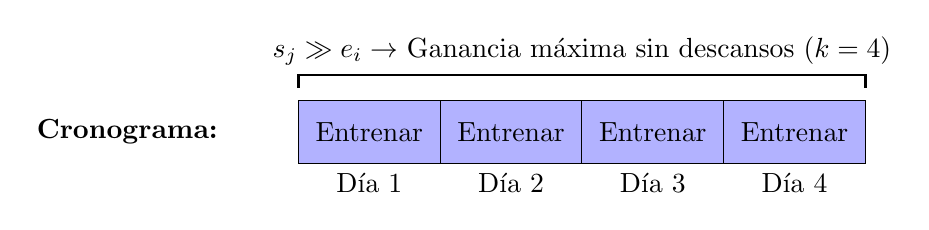
\begin{tikzpicture}[x=1.8cm, y=0.8cm]
            \node[anchor=east, font=\bfseries] at (-0.5, 0.5) {Cronograma:};
            \draw[fill=blue!30] (0,0) rectangle (1,1) node[midway] {Entrenar};
            \draw[fill=blue!30] (1,0) rectangle (2,1) node[midway] {Entrenar};
            \draw[fill=blue!30] (2,0) rectangle (3,1) node[midway] {Entrenar};
            \draw[fill=blue!30] (3,0) rectangle (4,1) node[midway] {Entrenar};
            
            \node[below] at (0.5, 0) {Día 1};
            \node[below] at (1.5, 0) {Día 2};
            \node[below] at (2.5, 0) {Día 3};
            \node[below] at (3.5, 0) {Día 4};
            
            \draw[thick] (0,1.2) -- (0,1.4) -- (4,1.4) -- (4,1.2);
            \node[above] at (2, 1.4) {$s_j \gg e_i \rightarrow$ Ganancia máxima sin descansos ($k=4$)};
        \end{tikzpicture}
    \end{figure}

    \item \textbf{Caso B: Caída abrupta de energía.}
    \begin{itemize}
        \item \textbf{Descripción:} El equipo sufre de fatiga extrema muy rápido. Por ejemplo, la energía inicial $s_1$ tiene un valor alto, pero para el segundo día consecutivo ($s_2$) decae abruptamente a valores cercanos a $0$.
        \item \textbf{Análisis:} Si la energía se desploma al segundo día de entrenamiento, cualquier bloque de tamaño $k \ge 2$ sumará un valor marginal en sus últimos días. Al algoritmo le resultará matemáticamente mucho más rentable insertar un día de descanso para resetear la fatiga y volver a aprovechar el alto valor de $s_1$. En consecuencia, la estructura del cronograma será una secuencia fragmentada, alternando estrictamente días de entrenamiento cortos (bloques de $k=1$) con días de descanso.
    \end{itemize}

    \begin{figure}[H]
        \centering
        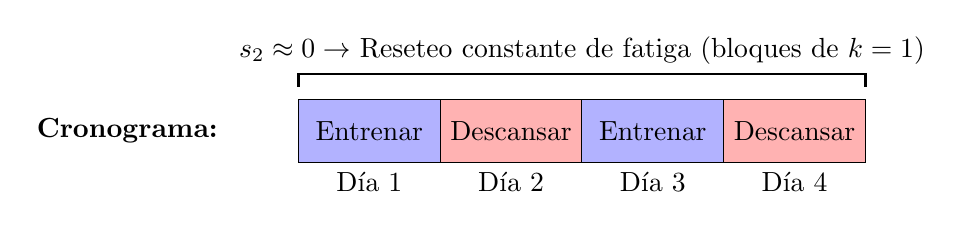
\begin{tikzpicture}[x=1.8cm, y=0.8cm]
            \node[anchor=east, font=\bfseries] at (-0.5, 0.5) {Cronograma:};
            \draw[fill=blue!30] (0,0) rectangle (1,1) node[midway] {Entrenar};
            \draw[fill=red!30]  (1,0) rectangle (2,1) node[midway] {Descansar};
            \draw[fill=blue!30] (2,0) rectangle (3,1) node[midway] {Entrenar};
            \draw[fill=red!30]  (3,0) rectangle (4,1) node[midway] {Descansar};
            
            \node[below] at (0.5, 0) {Día 1};
            \node[below] at (1.5, 0) {Día 2};
            \node[below] at (2.5, 0) {Día 3};
            \node[below] at (3.5, 0) {Día 4};
            
            \draw[thick] (0,1.2) -- (0,1.4) -- (4,1.4) -- (4,1.2);
            \node[above] at (2, 1.4) {$s_2 \approx 0 \rightarrow$ Reseteo constante de fatiga (bloques de $k=1$)};
        \end{tikzpicture}
    \end{figure}

\end{enumerate}

\subsection{Comportamiento en Programación Dinámica (Bottom-Up) vs. Reconstrucción (Top-Down)}

En contextos de alta variabilidad que generan empates sistemáticos (como en el Caso C), el impacto se debe interpretar de manera distinta según la fase del algoritmo:

\begin{itemize}
    \item \textbf{Fase Bottom-Up (Llenado del arreglo $OPT$):} La variabilidad y la multiplicidad de opciones \textbf{no afectan en lo absoluto el cálculo del valor óptimo}. Cuando la función $\max$ de la ecuación de recurrencia evalúa diferentes tamaños de bloque $k$ y descubre que varios devuelven el mismo puntaje máximo, la ecuación simplemente asimila ese número. El valor final acumulado que llegará a $OPT(n)$ será único, robusto y representará la ganancia teórica inamovible, a prueba de cualquier volatilidad en los datos de entrada.
    
    \item \textbf{Fase Top-Down (Algoritmo de Reconstrucción):} Aquí es donde la alta variabilidad tiene un impacto real y directo. Si durante la fase \textit{Bottom-Up} existieron múltiples valores de $k$ que empataron como el máximo para un mismo día $i$, significa que existen \textbf{múltiples cronogramas estructuralmente distintos que logran exactamente la misma ganancia total}. 
    
    Un algoritmo de reconstrucción típico almacena solo un valor de $k$ ganador por celda para lograr una complejidad de $\mathcal{O}(n)$. La decisión de \textit{cuál} $k$ se guarda ante un empate depende de un simple operador lógico en la implementación: si el código utiliza un comparador estricto ($>$), conservará el primer $k$ que encuentre; si utiliza mayor o igual ($\geq$), sobrescribirá la variable y se quedará con el último $k$ óptimo evaluado. 
    
    Por lo tanto, ante datos que generan empates constantes, el cronograma específico devuelto (el detalle de qué días puntuales se entrena o se descansa) puede variar diametralmente de una ejecución a otra o entre distintas implementaciones del mismo algoritmo, \textbf{aunque todas esas versiones representen caminos 100\% óptimos}.
\end{itemize}